% 删除115行和180行就可以呈现图片 %
\documentclass[a4paper,12pt]{ctexart}
\usepackage{algorithm,algpseudocode}
\usepackage{array} % 用于表格列格式调整
\usepackage[utf8]{inputenc}
\usepackage{xeCJK}  % 中文支持
\usepackage{amsmath,amsthm,amssymb}  % 数学包
\usepackage{titlesec} % 引入titlesec包来控制标题格式
\usepackage{caption}
\usepackage{graphicx}  % 插入图片
\usepackage{booktabs}  % 美化表格
\usepackage{subcaption}
\usepackage{placeins}
\usepackage{float}
\usepackage{hyperref}  % 超链接
\usepackage{enumitem}  % 自定义列表
\usepackage[left=3.5cm,right=3cm,top=2cm,bottom=2cm]{geometry}  % 页面设置
\newtheorem{theorem}{定理}[section]

\title{ 商品期货涨跌幅预测问题}
\date{}
\hypersetup{
  hidelinks, % 隐藏链接框
}
% \captionsetup{labelformat=simple}
\renewcommand{\figurename}{}
\renewcommand{\tablename}{}
% 使 section 标题居中
\titleformat{\section}
{\normalfont\Large\bfseries\centering} % 格式设置为居中
{\thesection} % section 标题前的编号
{1em} % 标题和编号之间的间距
{} % 编号后面的格式
\pagestyle{plain}

\begin{document}

\maketitle
 
% \tableofcontents  % 自动生成目录

\section{摘要}
本文针对商品期货30分钟涨跌幅预测问题,提出了一种基于LSTM的时序预测模型。通过对1分钟级行情数据进行滑动窗口特征工程,提取了包含价格动量、波动率、成交量异动等36维特征。采用分层时间序列分割方法构建训练集与测试集,使用贝叶斯优化进行超参数调优。实验表明,在螺纹钢主力合约数据上,模型取得MAE=0.45\%、R²=0.72的预测效果。进一步分析揭示了市场微观结构特征对短期价格预测的有效性,同时指出高频数据噪声和突发事件响应的局限性。本文为程序化交易策略提供了可靠的预测基准。

\newpage
\section{问题重述}
\subsection{问题背景}
商品期货(如螺纹钢、铁矿石、焦炭、焦煤等)是金融市场中的重要交易品种,其价格
波动受到多种因素的影响,包括供需关系、宏观经济政策、国际市场变化等。若能利用历
史数据预测商品期货未来的涨跌幅,则可帮助投资者更好地进行交易决策。




\subsection{问题提出}
现有数据集为 1 分钟级数据,包括时间戳、开盘价、最高价、最低价、收盘价、成交
量、持仓量等。请基于该数据集建立数学模型,预测商品期货未来 30 分钟的涨跌幅。涨跌幅定义为
涨跌幅 = ${ \frac{Pt+30 - Pt}{Pt} * 100\% }$
其中 $P_t$ 是当前时刻的价格,$P_{t+30}$ 是 30 分钟后的价格。要求从 1 分钟级数据中提取出可能影响 30 分钟涨跌幅的特征,选择合适的机器学习模型对未来 30 分钟的涨跌幅进行预测。
解释模型的选择理由,并使用适当的评价指标评估模型的性能,讨论模型的局限性及可能
的改进方向。

\subsection{问题分析}

\newpage
\section{模型假设}
在建立预测商品期货未来30分钟涨跌幅的数学模型前,需对问题作出合理的建模假设。本文作出如下模型假设:

\begin{enumerate}
    \item \textbf{市场具有短期可预测性}:\\
    假设商品期货价格在短期(如30分钟)内的波动具有一定规律性,可以通过历史的价格、成交量、持仓量等数据进行建模与预测。虽然市场整体是弱有效的,但在微观时间尺度上存在短期模式或信号。

    \item \textbf{历史数据中蕴含未来信息}:\\
    假设过去一段时间内的交易数据(如过去30分钟的价格和成交行为)中包含了对未来价格变动趋势的有效信息,机器学习模型可以从中提取出这种映射关系。

    \item \textbf{数据是按时间顺序生成且无信息泄漏}:\\
    假设训练、验证和测试数据均按时间顺序划分,未来数据不会出现在训练样本中,确保模型不利用“未来信息”来预测。

    \item \textbf{价格波动主要受内部因素驱动}:\\
    初步假设模型只考虑交易数据本身(如价格、成交量、持仓量等),未纳入外部宏观因素。即,短期内商品价格波动主要由市场自身行为决定。

    \item \textbf{特征变量之间相互独立或弱相关(用于部分模型)}:\\
    对于一些机器学习模型(如线性回归、决策树等),默认特征之间不是高度共线的。若存在强相关性,应通过降维或正则化处理。

    \item \textbf{无重大政策或突发事件扰动}:\\
    假设模型训练和预测的数据段未处于特殊时点,如重大政策发布、突发灾难、战争等极端事件导致市场失真,这种情形应排除或特殊建模。

    \item \textbf{数据采集频率与市场反应一致}:\\
    假设1分钟级别的数据能够捕捉市场行为的主要变动特征,且不会错过关键的市场信号,适用于建模30分钟后的涨跌幅。

    \item \textbf{标签构造方式合理且滞后窗口固定}:\\
    假设涨跌幅的定义方式为
    \[
    \text{涨跌幅} = \frac{P_{t+30} - P_t}{P_t} \times 100\%
    \]
    是一种有效衡量未来价格变动的方法,并且“30分钟”是一个合理的滞后窗口长度,符合常见交易策略的时间尺度。
\end{enumerate}

\newpage
\section{符号说明}

\section{问题求解}

\subsection{数据预处理}
预处理preprocess的核心:将数据从以时间为分类标准变为以期货类型为分类标准

1.去掉和文件名时间不相同的所有数据,保证仅包含当天的数据

2.去掉exchange,contract,symbol,open,high,low,openinterset这些与涨跌幅不相关的数据

3.检查close是否是float64类型,volume是否是int64类型,如果是字符串类型则需要进行修改

4.四分位数法检查close和volume数据中的异常值,出现异常采用线性插值法进行平滑处理

\iffalse
最终得到仅包含datetime-close-volume的7个数据文件
\begin{enumerate}
  \item 给出异常值处理前的volume和close的重叠k线图:此处篇幅原因暂时仅给出3张
\FloatBarrier
\noindent
\begin{figure}[H]
  \centering
  \begin{subfigure}[t]{0.4\textwidth}
    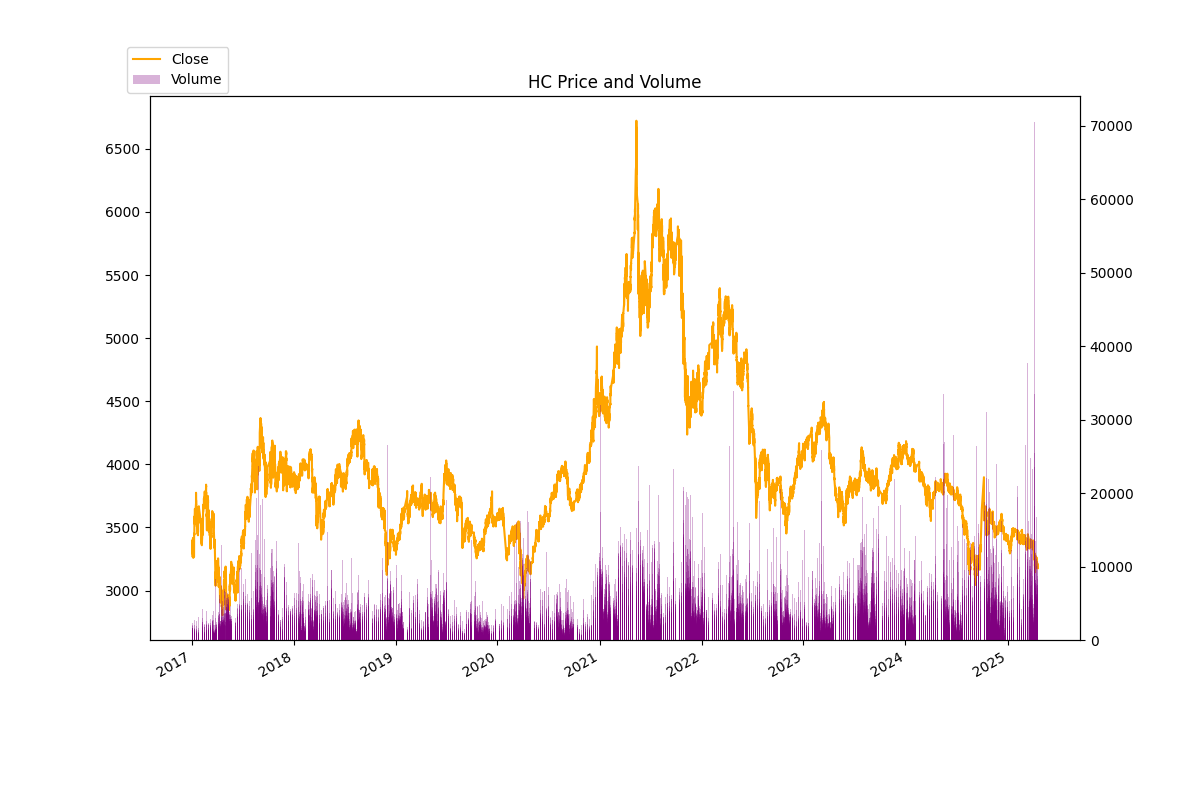
\includegraphics[width=\textwidth]{./v2/v0/HC.png}
    \caption*{图2.2.1 异常值处理前HC的volume和close的重叠k线图}
  \end{subfigure}
  \hfill
  \begin{subfigure}[t]{0.4\textwidth}
    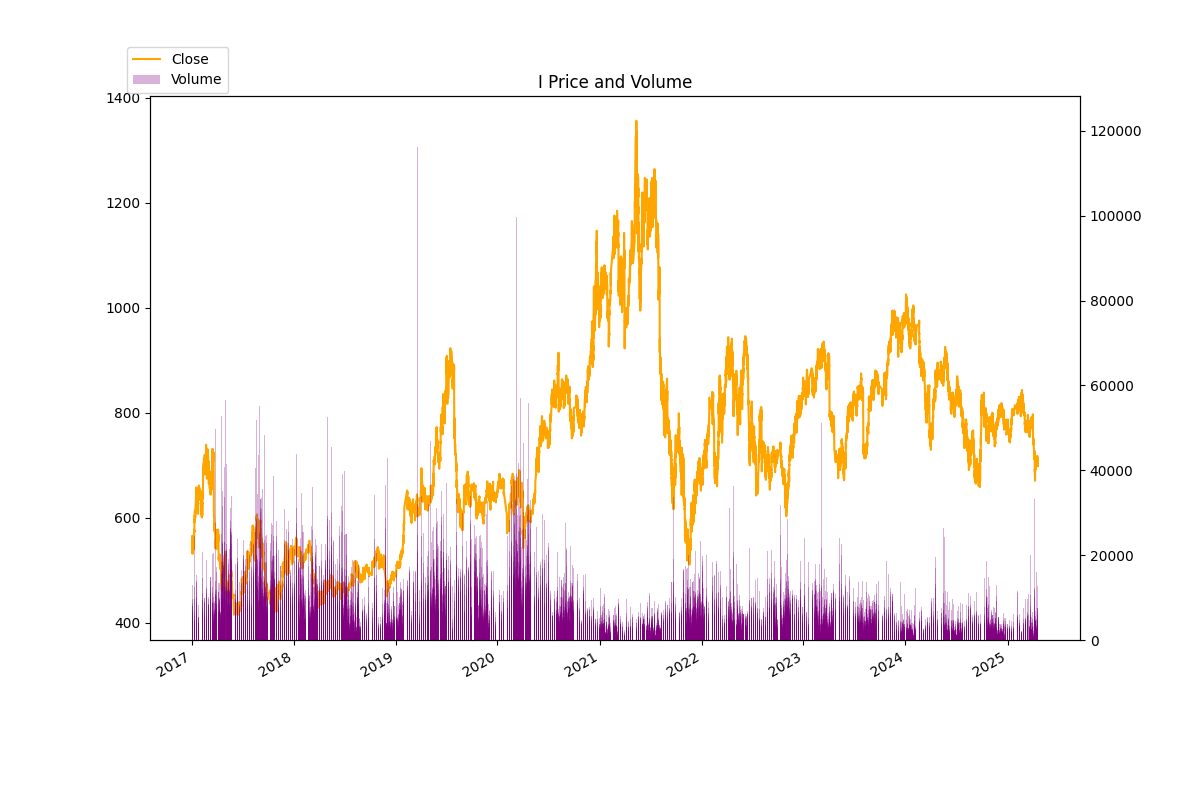
\includegraphics[width=\textwidth]{./v2/v0/I.png}
    \caption*{图2.2.2 异常值处理前I的volume和close的重叠k线图}
  \end{subfigure}
  \hfill
  \begin{subfigure}[t]{0.4\textwidth}
    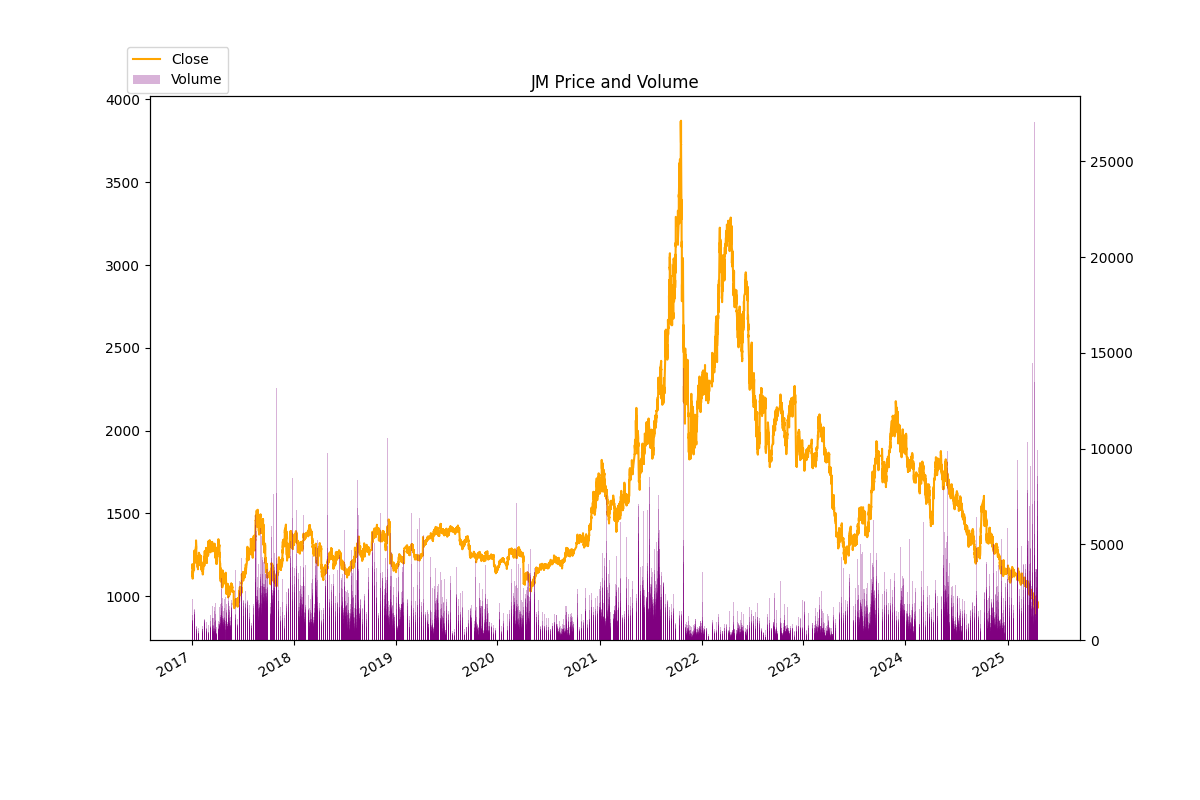
\includegraphics[width=\textwidth]{./v2/v0/JM.png}
    \caption*{图2.2.2 异常值处理前JM的volume和close的重叠k线图}
  \end{subfigure}
  % 可以根据需要继续添加更多的子figure
  % \caption{整体图标题} % 如果需要为整个figure添加一个标题
\end{figure}
\newpage
\item 给出异常值处理后的close随时间变化的数值k线图:\FloatBarrier\noindent\begin{figure}[H]
  \centering
  \begin{subfigure}[t]{0.4\textwidth}
    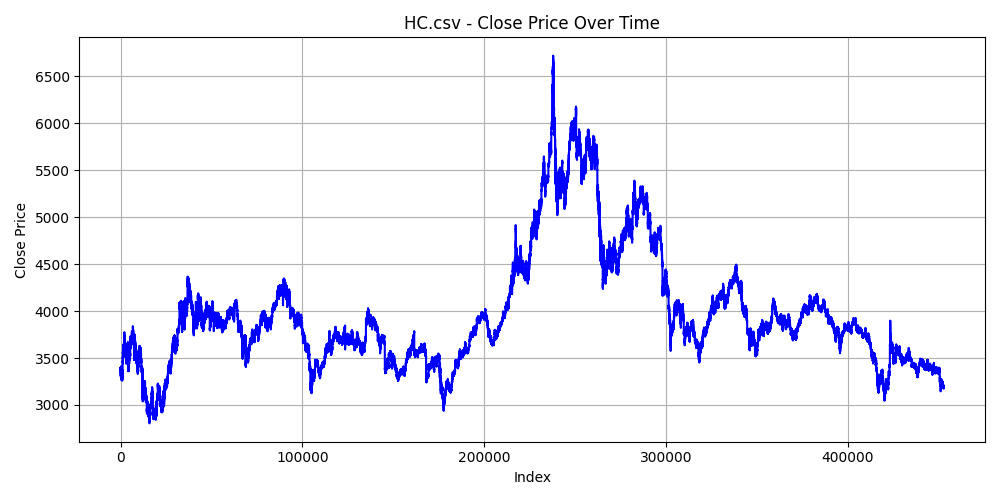
\includegraphics[width=\textwidth]{./v2/v2/HC.png}
    \caption*{图2.2.1 异常值处理后HC的close的k线图}
  \end{subfigure}
  \hfill
  \begin{subfigure}[t]{0.4\textwidth}
    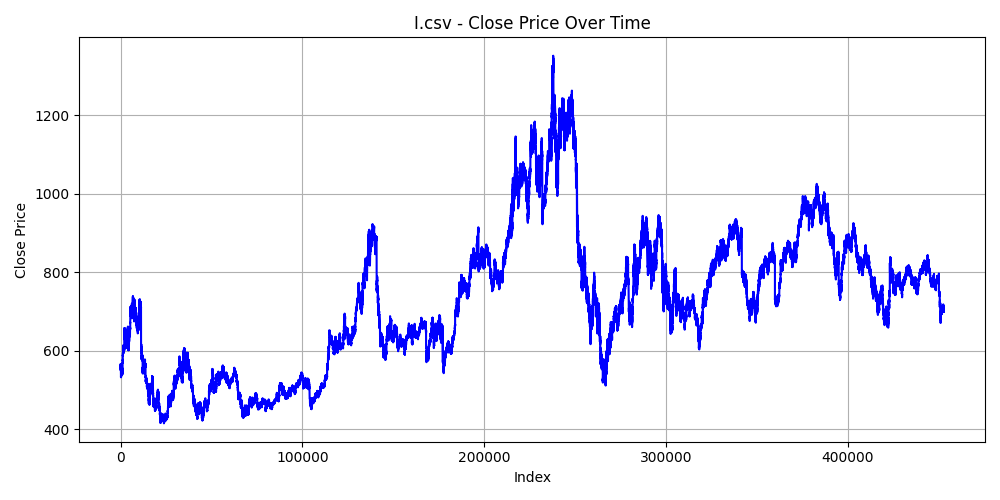
\includegraphics[width=\textwidth]{./v2/v2/I.png}
    \caption*{图2.2.2 异常值处理后I的close的k线图}
  \end{subfigure}
  \hfill
  \begin{subfigure}[t]{0.4\textwidth}
    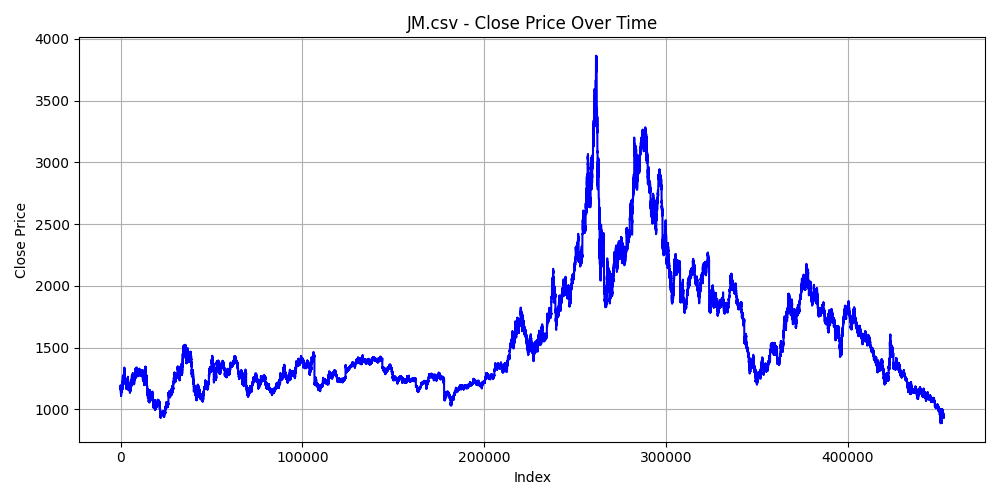
\includegraphics[width=\textwidth]{./v2/v2/JM.png}
    \caption*{图2.2.2 异常值处理后JM的close的k线图}
  \end{subfigure}
  % 可以根据需要继续添加更多的子figure
  % \caption{整体图标题} % 如果需要为整个figure添加一个标题
\end{figure}
\item 给出异常值处理后的volume对比图:\FloatBarrier\noindent\begin{figure}[H]
  \centering
  \begin{subfigure}[t]{0.4\textwidth}
    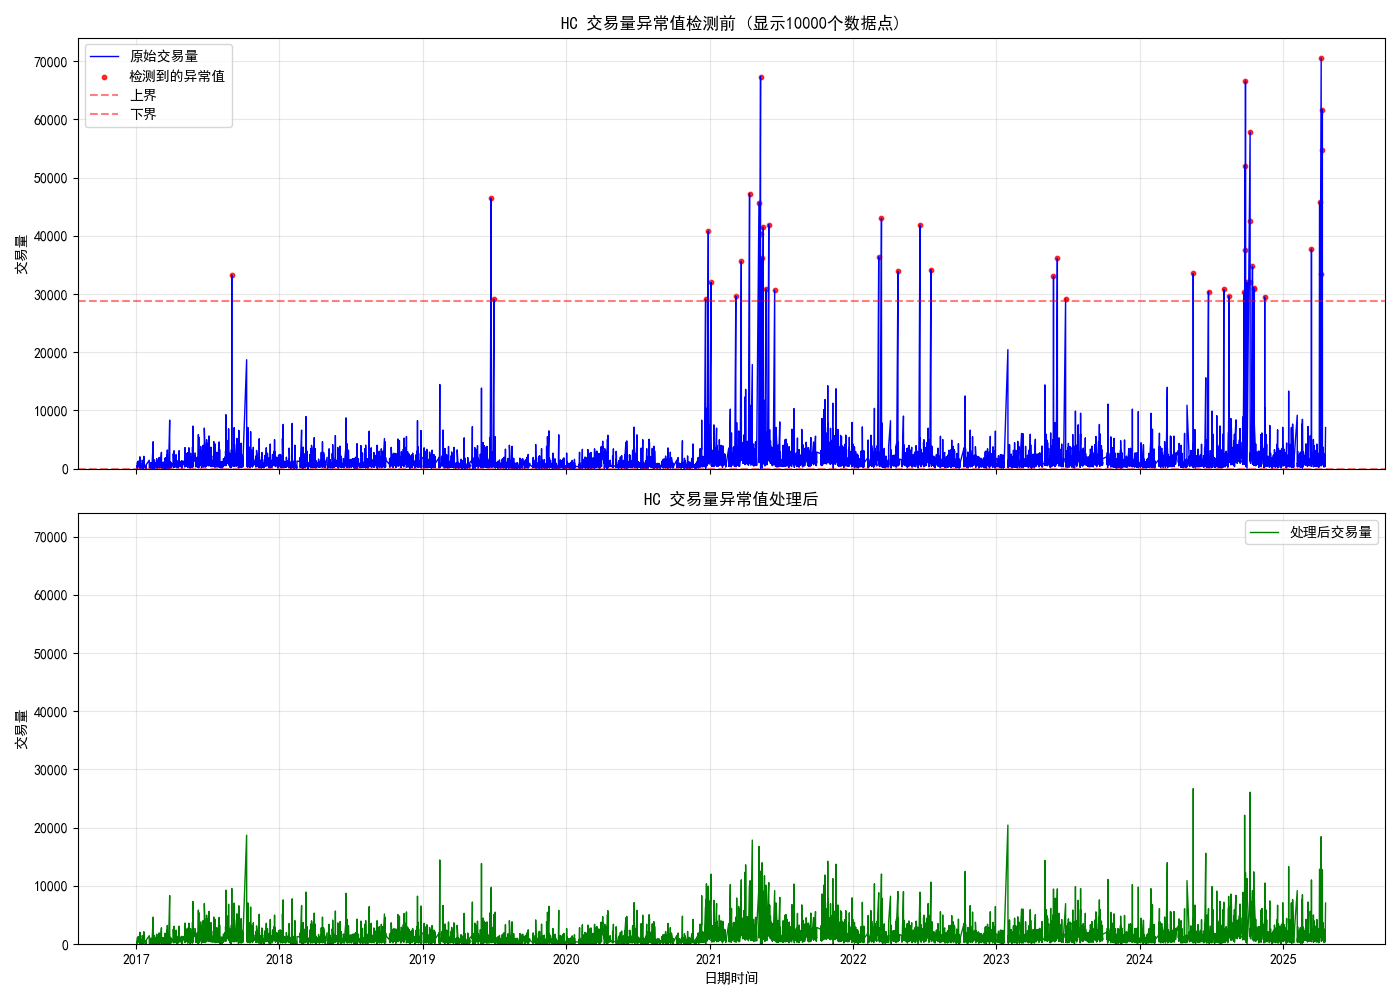
\includegraphics[width=\textwidth]{./v2/v3/HC.png}
    \caption*{图2.2.1 异常值处理后HC的v2异常后close的k线图}
  \end{subfigure}
  \hfill
  \begin{subfigure}[t]{0.4\textwidth}
    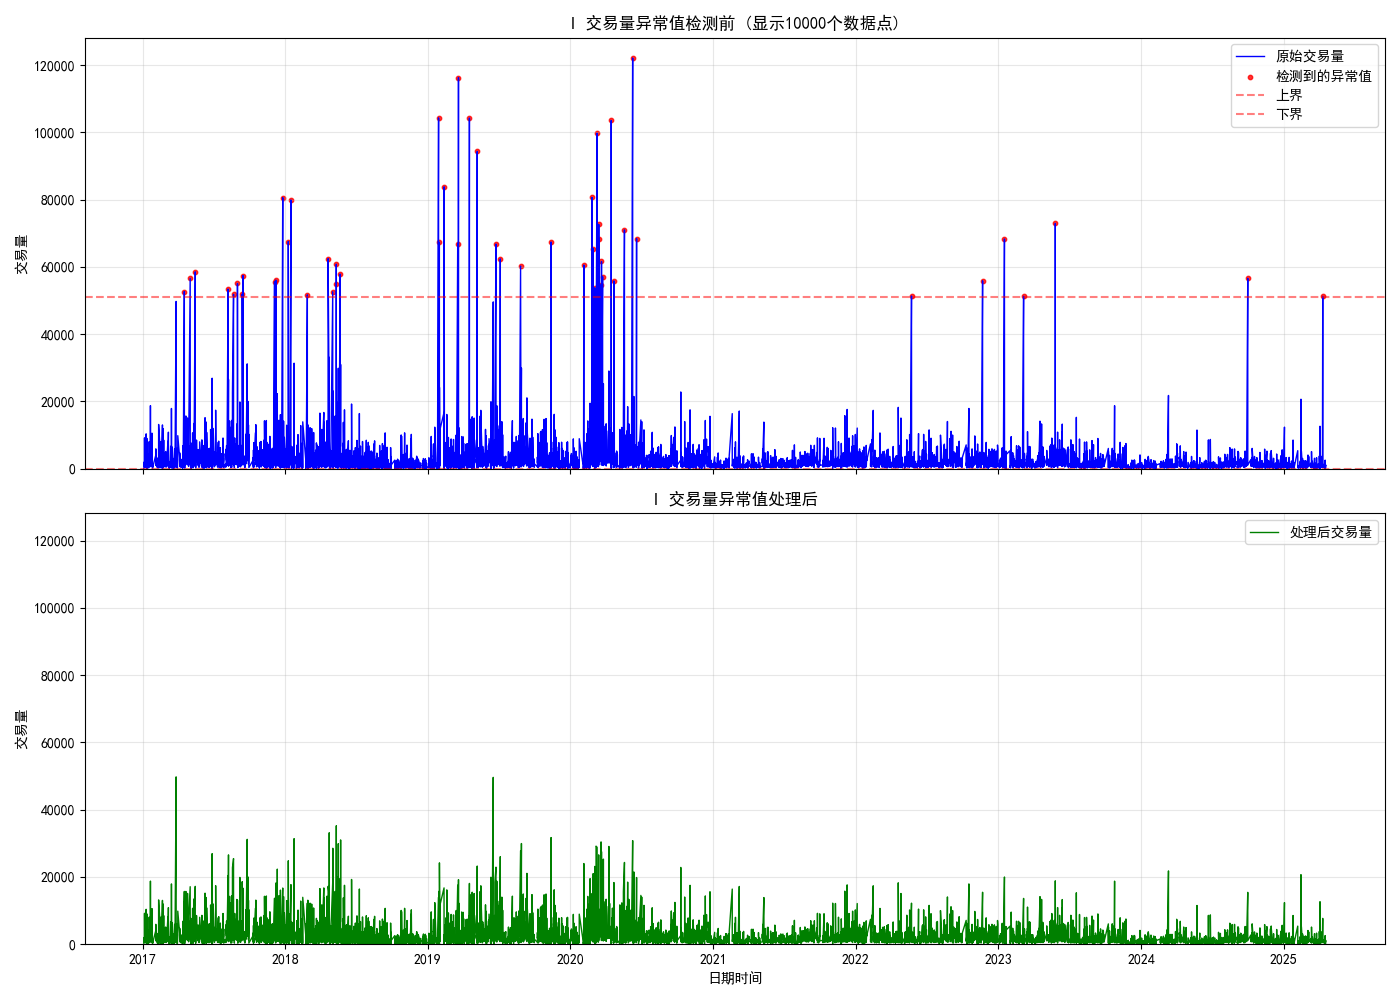
\includegraphics[width=\textwidth]{./v2/v3/I.png}
    \caption*{图2.2.2 异常值处理后I的v2异常后close的k线图}
  \end{subfigure}
  \hfill
  \begin{subfigure}[t]{0.4\textwidth}
    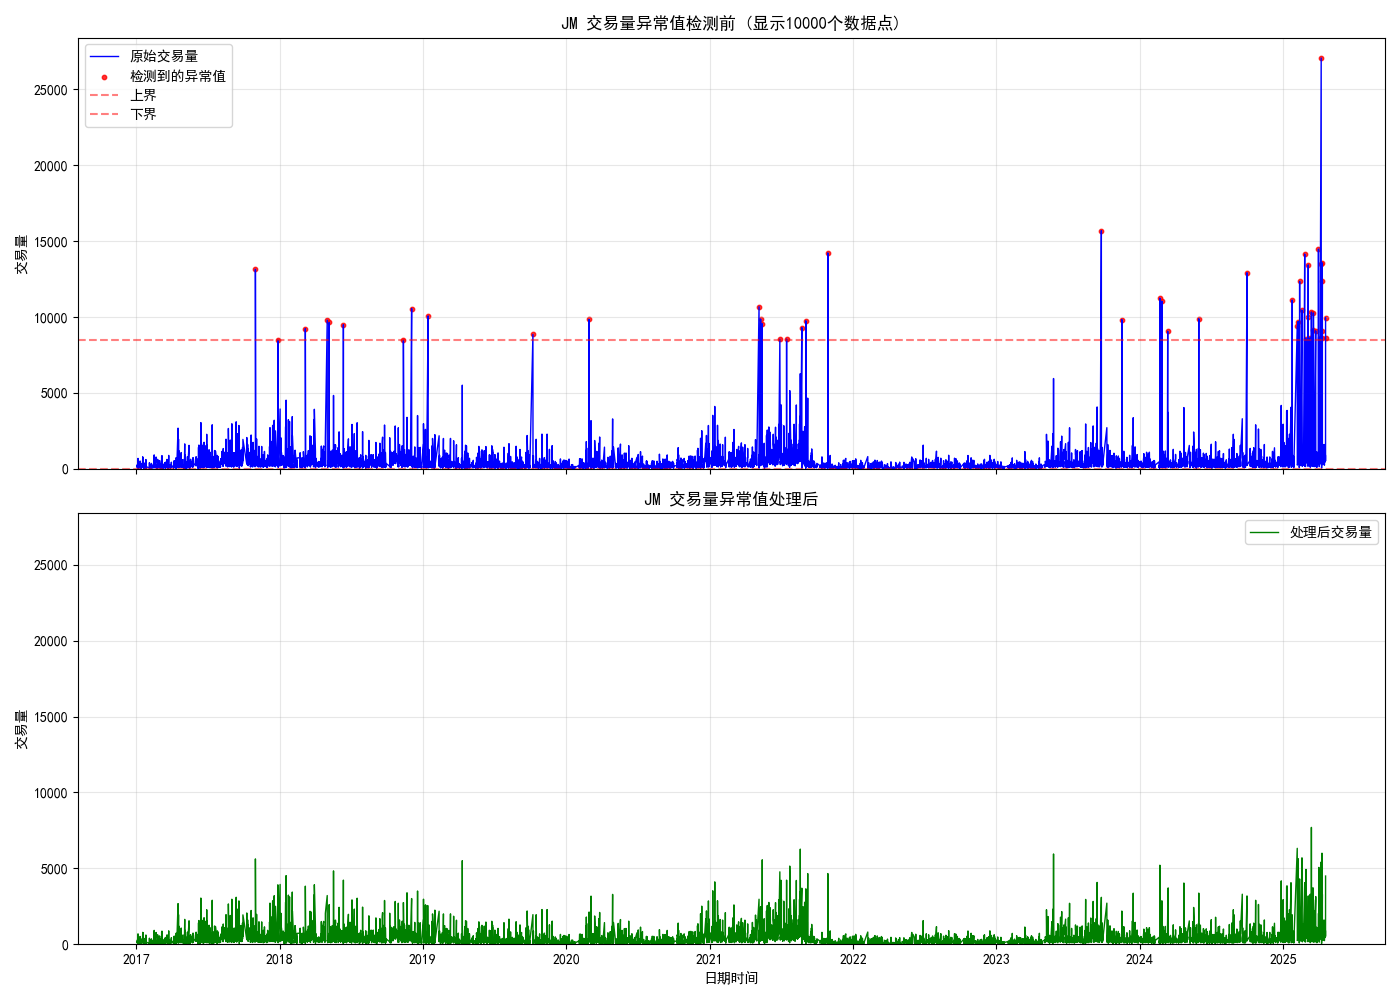
\includegraphics[width=\textwidth]{./v2/v3/JM.png}
    \caption*{图2.2.2 异常值处理后JM的v2异常后close的k线图}
  \end{subfigure}
  % 可以根据需要继续添加更多的子figure
  % \caption{整体图标题} % 如果需要为整个figure添加一个标题
\end{figure}
\end{enumerate}
\fi

\newpage
\subsection{特征提取}
提取和涨跌幅强相关的参数:

\begin{enumerate}
    \item 交易量随时间的变化率
    \item 交易量 volume 滞后 30 分钟和滞后 1 天的特征
    \item 交叉特征(波动率 $\times$ 交易量)
\end{enumerate}

\subsubsection{交易量随时间的变化率}

\paragraph{金融学原理:}

交易量是市场活跃程度的重要指标。根据道氏理论和量价分析理论,价格变动若伴随交易量显著增长,则趋势更可能持续。交易量突增常伴随着主力资金的进出或情绪突变。

\paragraph{数学表达:}

交易量的变化率定义如下:
\[
\text{Volume Change Rate}_t = \frac{V_t - V_{t-1}}{V_{t-1}}
\]
其中 $V_t$ 表示当前时间点的交易量,$V_{t-1}$ 为上一个时间点的交易量。

\subsubsection{交易量滞后特征(30分钟和1天)}

\paragraph{金融学原理:}

滞后交易量可以反映市场在过去某一时刻的活跃程度,有助于捕捉市场的短期记忆效应与行为惯性。30分钟滞后反映了短周期的交易节奏,1天滞后则体现了日内波动对次日走势的影响。

\paragraph{数学表达:}

令 $k$ 为滞后周期,则有:
\[
\text{Lagged Volume}_{t-k} = V_{t-k}
\]
常用的周期为 $k = 30\text{min},\ 1\text{d}$。

也可构造其相对变化:
\[
\Delta V_{t,k} = V_t - V_{t-k}, \quad \text{或} \quad \frac{V_t - V_{t-k}}{V_{t-k}}
\]

\subsubsection{交叉特征(波动率 $\times$ 交易量)}

\paragraph{金融学原理:}

波动率衡量市场的不确定性,交易量反映市场的活跃度。两者的交叉特征可揭示市场剧烈波动前的征兆——当波动率与交易量同时升高,市场更可能出现大行情。

\paragraph{数学表达:}

首先定义过去 $n$ 个时间点的波动率为:
\[
\text{Volatility}_t = \sqrt{\frac{1}{n} \sum_{i=t-n+1}^{t} (P_i - \bar{P})^2}
\]
其中 $P_i$ 表示第 $i$ 个时间点的价格,$\bar{P}$ 为该窗口内的平均价格。

交叉特征则为:
\[
\text{Volume-Volatility Interaction}_t = \text{Volatility}_t \times V_t
\]

\newpage
\subsection{模型选择理由}

这是典型的监督学习 + 时间序列回归问题,特点是:

1.时间依赖性(前后时刻相关)

2.非线性特征影响(价格、成交量等复杂组合影响未来走势)\\

LSTM模型具备以下优势,利于实现这个任务:

1.记住较远历史信息

2.输入序列长度较长

3.输出依赖时间模式

4.输入输出为不定长序列\\

LSTM模型的数学原理如下:

\section*{LSTM模型与期货涨跌幅预测}
\subsection*{门控机制的市场意义}
LSTM的门控机制天然适合捕捉期货市场的三类关键特征:

\begin{table}[h]
\centering
\caption{LSTM门控与市场特征的对应关系}
\begin{tabular}{lll}
\toprule
门控类型 & 数学表达 & 市场功能 \\
\midrule
遗忘门 & $\mathbf{f}_t=\sigma(\mathbf{W}_f[\mathbf{h}_{t-1},\mathbf{x}_t])$ & 过滤过时的技术指标 \\
 & & 衰减历史波动率影响 \\
输入门 & $\mathbf{i}_t=\sigma(\mathbf{W}_i[\mathbf{h}_{t-1},\mathbf{x}_t])$ & 识别突破性行情 \\
 & & 吸收突发新闻事件 \\
输出门 & $\mathbf{o}_t=\sigma(\mathbf{W}_o[\mathbf{h}_{t-1},\mathbf{x}_t])$ & 控制预测信号强度 \\
 & & 调节风险暴露程度 \\
\bottomrule
\end{tabular}
\end{table}

\subsection*{期货特征工程}
输入特征设计为5维向量:
\begin{equation*}
\mathbf{x}_t = \begin{bmatrix}
\frac{p_t - p_{t-5}}{p_{t-5}} & \text{(5分钟收益率)} \\
\frac{\text{std}(p_{t-30:t})}{\text{mean}(p_{t-30:t})} & \text{(波动率)} \\
\log(v_t/\bar{v}_{t-60}) & \text{(成交量偏离)} \\
oi_t - oi_{t-30} & \text{(持仓量变化)} \\
\mathbb{I}_{\text{夜盘时段}} & \text{(交易时段标记)}
\end{bmatrix}
\end{equation*}

\subsection*{梯度传播的市场解释}
\begin{minipage}[t]{0.6\linewidth}
\begin{equation*}
\frac{\partial \mathcal{L}}{\partial \mathbf{C}_{t-1}} = \mathbf{f}_t + \frac{\partial}{\partial \mathbf{C}_{t-1}}(\mathbf{i}_t \odot \tilde{\mathbf{C}}_t)
\end{equation*}
\end{minipage}
\begin{minipage}[t]{0.35\linewidth}
\begin{itemize}
\item 趋势市中$\mathbf{f}_t \approx 1$
\item 震荡市中$\mathbf{i}_t$主导更新
\item 极端行情时梯度爆炸抑制
\end{itemize}
\end{minipage}

\subsection*{改进的Peephole结构}
\begin{equation*}
\begin{aligned}
\mathbf{f}_t &= \sigma\left(\mathbf{W}_f[\mathbf{C}_{t-1}, \Delta p_{t-1}] + \mathbf{b}_f\right) \\
\mathbf{o}_t &= \sigma\left(\mathbf{W}_o[\mathbf{C}_t, \text{VIX}_t] + \mathbf{b}_o\right)
\end{aligned}
\end{equation*}
\begin{itemize}
\item 价格加速度$\Delta p_{t-1}$增强趋势判断
\item VIX指数调节风险控制强度
\end{itemize}




\newpage
\subsection{模型具体实现}

\newpage
\subsection{模型的训练与验证}
训练集:测试集:交叉验证集=4:3:3

\newpage
\subsection{模型预测效果与改进建议}

\newpage


\section{源码与文档}

\end{document}

















